\documentclass[]{article}
\usepackage{lmodern}
\usepackage{float}
\usepackage{amssymb,amsmath}
\usepackage{ifxetex,ifluatex}
\usepackage{fixltx2e} % provides \textsubscript
\ifnum 0\ifxetex 1\fi\ifluatex 1\fi=0 % if pdftex
  \usepackage[T1]{fontenc}
  \usepackage[utf8]{inputenc}
\else % if luatex or xelatex
  \ifxetex
    \usepackage{mathspec}
  \else
    \usepackage{fontspec}
  \fi
  \defaultfontfeatures{Ligatures=TeX,Scale=MatchLowercase}
\fi
% use upquote if available, for straight quotes in verbatim environments
\IfFileExists{upquote.sty}{\usepackage{upquote}}{}
% use microtype if available
\IfFileExists{microtype.sty}{%
\usepackage{microtype}
\UseMicrotypeSet[protrusion]{basicmath} % disable protrusion for tt fonts
}{}
\usepackage[unicode=true]{hyperref}
\hypersetup{
            pdftitle={I/O analysis of climate applications},
            pdfauthor={Arne Beer, MN 6489196, Frank Röder, MN 6526113},
            pdfborder={0 0 0},
            breaklinks=true}
\urlstyle{same}  % don't use monospace font for urls
\usepackage{graphicx,grffile}
\makeatletter
\def\maxwidth{\ifdim\Gin@nat@width>\linewidth\linewidth\else\Gin@nat@width\fi}
\def\maxheight{\ifdim\Gin@nat@height>\textheight\textheight\else\Gin@nat@height\fi}
\makeatother
% Scale images if necessary, so that they will not overflow the page
% margins by default, and it is still possible to overwrite the defaults
% using explicit options in \includegraphics[width, height, ...]{}
\setkeys{Gin}{width=\maxwidth,height=\maxheight,keepaspectratio}
\IfFileExists{parskip.sty}{%
\usepackage{parskip}
}{% else
\setlength{\parindent}{0pt}
\setlength{\parskip}{6pt plus 2pt minus 1pt}
}
\setlength{\emergencystretch}{3em}  % prevent overfull lines
\providecommand{\tightlist}{%
  \setlength{\itemsep}{0pt}\setlength{\parskip}{0pt}}
\setcounter{secnumdepth}{0}
% Redefines (sub)paragraphs to behave more like sections
\ifx\paragraph\undefined\else
\let\oldparagraph\paragraph
\renewcommand{\paragraph}[1]{\oldparagraph{#1}\mbox{}}
\fi
\ifx\subparagraph\undefined\else
\let\oldsubparagraph\subparagraph
\renewcommand{\subparagraph}[1]{\oldsubparagraph{#1}\mbox{}}
\fi

\title{I/O analysis of climate applications}
\author{Arne Beer, MN 6489196, Frank Röder, MN 6526113}
\date{}

\begin{document}
\maketitle

{
\setcounter{tocdepth}{3}
\tableofcontents
}
\pagebreak

\section{Introduction}\label{introduction}

\subsection{About the paper and our
goals}\label{about-the-paper-and-our-goals}

In this paper we analyze and present the strengths and weaknesses of
different data structures required by some carefully picked climate and
weather prediction models. Further we investigate the bare minimum of
data required by those models. Another important aspect we will
elaborate is the pre- and post-processing of data and the precise moment
it occurs.

In the following sections we will elucidate some models and the process
on how to set them up as well as running sample cases. At the end there
will be a section about the overall life cycle of data.

\subsection{Getting started}\label{getting-started}

With intent of getting an overview about the richness of climate
applications and their land, ice, weather and ocean modulation, we took
an in-depth look at some models. The main goal was to find a model with
proper documentation and a license which allowed us to use it for our
research and benchmarking purposes. Most model investigated by us were
too old for our objective. In many cases there were practically no
documentation, let alone active support or new releases. The next
obvious step was to get an good overview of up to date and easy to
handle models which are still supported. For this purpose we put a
spreadsheet together from which we could choose the most promising ones.
We came across some good looking models, but despite a good first
impression, most of them are shipped with broken scripts, bad
documentation or a hidden provision, which forbids us to use them. After
a long trial and error period of testing new models, we finally decided
to stick to two models, which will be addressed later in this paper.

\pagebreak

\section{IFS - Integrated Forecasting
System}\label{ifs---integrated-forecasting-system}

\subsection{About IFS}\label{about-ifs}

\emph{IFS} has been chosen to be the first model for our research.
\emph{IFS} is a Model created and used by the European Center for
Medium-range Weather Forecast (ECMWF). The purpose of this model is to
create weather predictions by analyzing a huge amount of data. This data
can be a variety of different physical bulks. \cite{ifs}

\textbf{ECMWF} offers a semi open-source version of their model for
research institutions, which is called \emph{OpenIFS}. The source code
of this model can be obtained by requesting a license for the
institution one is working for. They provide a good documentation about
their model, which covers instruction for building, running simulations
as well as very detailed information about the mathematics and
techniques used in their model. After some research and two weeks
passing by, we discovered a passage in their license, which forbids
``Commercial and benchmarking use of \emph{OpenIFS} models''. As our
original research goal is some kind of benchmarking we were forced to
stop and switch to another model. We still recommend to use this model
in a research or academic context, as there is plenty of documentation
and a big user base.

\pagebreak

\section{Further progress}\label{further-progress}

After the license incident with IFS we had to look for other open source
models we could use for our research. We looked at many models in the
following we will list some of the most promising:

\begin{itemize}
\tightlist
\item
  WRF(The Weather Research \& Forcasting Model)
\item
  CFS(Climate Forecast System)
\item
  GDAS (Global Data Assimilation System)
\item
  GFS (Global Forecast System)
\item
  GEFS(Global Ensemble Forecast System)
\item
  CM2.X (CM2 Global Coupled Climate Models)
\item
  GISS GCM ModelE
\item
  \emph{CESM}(Community Earth System Model)
\item
  MITgcm (M.I.T. General Circulation Model News and Information)
\item
  GEOSCI (Geoscientific Model Development)
\item
  Hector v1.0
\item
  MAGICC/SCENGEN (Model for the Assessment of Greenhouse-gas Inducted
  Climate Change A Regional Climate SCENario GENerator)
\item
  Metview
\item
  COSMO(Consortium For Small Scale Modeling)
\item
  SAGA (System for Automated Geoscientific Analyses)
\item
  MPI-ESM
\item
  ECOHAM
\end{itemize}

The lookup for new models took about two weeks. Most of the models
mentioned above had serious flaws which forbid us to use them in our
research. Many of them have stopped being maintained many years ago. In
some cases there was no license provided with no available support for
clarifying legal questions. In other cases it was only possible to
obtain a license for our specific research goal by buying it or it was
even completely forbidden to use it for benchmarking purposes, as with
\emph{OpenIFS}.

Eventually we decided to focus our work on \emph{Community Earth System
Model} (\emph{CESM}) and Ecosystem model Hamburg Version 5 (ECOHAM5).
Further we decided to take a look at \emph{AWIPS2} a tool for displaying
processed weather forecast with a very good server for handling data
called \emph{EDEX} .

\pagebreak

\section{Unidata - AWIPS2}\label{unidata---awips2}

\emph{AWIPS2} contains tools for weather forecast displaying and
analysis. This open-source \texttt{Java} application consists of
\emph{EDEX} a data server and \emph{CAVE} the client for data analysis
and rendering. \cite{Uni01} Cite : ``AWIPS II is a Java application
consisting of a data display client \emph{CAVE} which runs on Red
Hat/CentOS Linux and OS X and a backend data server EDEX which only runs
on Linux'' \cite{Awips}

\begin{figure}
\centering
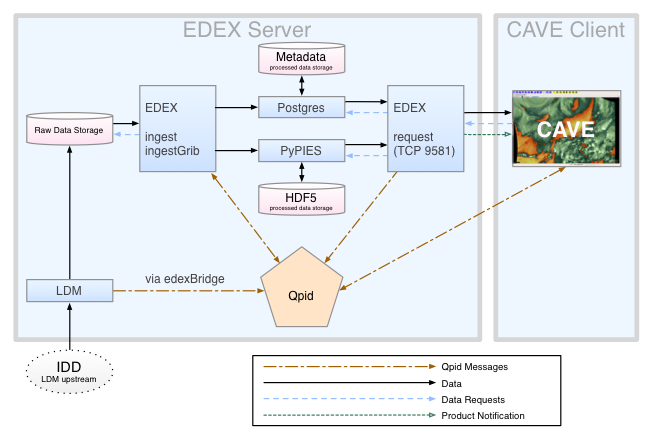
\includegraphics{pics/awips2_coms.png}
\caption{AWIPS2 System}
\end{figure}

\subsection{EDEX (Environmental Data EXchange
)}\label{edex-environmental-data-exchange}

\textbf{EDEX} is the server for \emph{AWIPS2} which is mainly used for
preparing the data needed by \emph{CAVE}. The \emph{EDEX} server is a
compound of different components: \cite{AwipsDocs}

The first source for data is the Local Data Manager (\emph{LDM}). This
is a piece of software which shares data with computers in other
networks. The Internet Data Distribution (\emph{IDD}) provides the
\emph{LDM} with data from the Unidata community. The \emph{LDM} can
handle different kinds of data, for instance National Weather Service
data streams, radar data, satellite images or grid data from numerical
forecast models. The data can be directly obtained from the source or by
a \emph{LDM} that communicates with another \emph{LDM}. When the
\emph{LDM} receives data inside the \emph{EDEX}, a message about
availability of new data is being send to the \textbf{Qipd} process, the
Apache \textbf{Queue Processor Interface Daemon}, which distributes it
to all other components of the \emph{EDEX} server. The messages from
\textbf{Qipd} will also contain a file header for \emph{EDEX} to know
which decoder should be used for the specific data.

After that \emph{EDEX} can decode the data to make it ready for
additional processing or signal \emph{CAVE} that it is available for
displaying. All of those messages are sent via the \textbf{edexBridge}.
The default ingest server will handle all the data which are different
to grib messages and is in general just responsible for the ingest of
data. GRIB fully spelled \textbf{General Regularly-distributed
Information in Binary form} is a data format by the \textbf{\emph{WMO}}
(World Meteorological Organization) and used for encoding results of
weather models. The data is written in a binary shape into a table
format. It is optimized for store and transfer data. The PostgreSQL
database or \textbf{Postgres} in short is another relevant part for the
storage of data in \emph{EDEX}. It handles the metadata of the already
decoded data. Postgres itself is a relational database management system
which reads and store all \emph{EDEX} metadata. The database size is not
limited and can handle 32 TB of database table capacity.

\emph{HDF5} fully spelled Hierarchical Data Format (v.5) is the main
format used in \emph{AWIPS2} to store processed grids, images, etc. .
Nowadays it is very similar to netCDF, which is supported by Unidata.
HDF5 can handle many different types of data in a single file, for
instance data of multiple radars.

The \textbf{Python Process Isolated Enhanced Storage} PyPIES has been
just created for \emph{AWIPS2} and is used for the writes and reads of
data in HDF5 files. \textbf{PyPIES} is very similar in functionality
compared to \textbf{Postgres}. It is a custom database abstraction
layer, which processes any requests related to the HDF5 file system. The
intention for this layer was to isolate the EDEX from the HDF5
processes.

\subsection{CAVE (Common AWIPS Visualization
Environment)}\label{cave-common-awips-visualization-environment}

\emph{CAVE} is the second part of \emph{AWIPS2}. It is a tool for data
visualization and rendering. Normally it is installed on a separated
workstation apart from the other \emph{AWIPS2} parts.\\
Cite: ``CAVE contains of a number of different data display
configurations called perspectives. Perspectives used in operational
forecasting environments include D2D (Display Two-Dimensional), GFE
(Graphical Forecast Editor), and NCP (National Centers Perspective).
\cite{AwipsDocs}

\begin{figure}
\centering
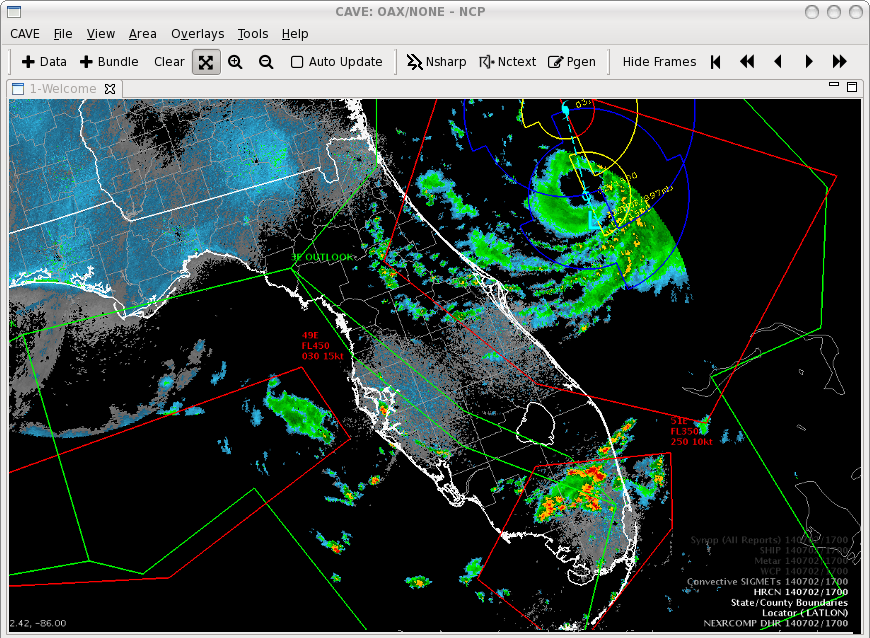
\includegraphics{pics/Unidata_AWIPS2_CAVE.png}
\caption{CAVE Example}
\end{figure}

\subsection{Installation}\label{installation}

For the installation of \emph{AWIPS2} UniData provides a Github
repository \url{https://github.com/Unidata/awips2} and two install
scripts \texttt{installCave.sh} and \texttt{installEDEX.sh}. Those
install scripts use yum as a package manager and are designed for usage
on CentOS, Fedora and Red Hat. To make it compatible for the \emph{DKRZ}
cluster there is more that needs to be done. As stated before
\emph{AWIPS2} is normally installed with the help of the package manager
YUM and \emph{AWIPS2} requires a directory at root location
``/awips2/''. There are about 2000 lines of code where ``/awips2/'' is
hard-coded, so switching directories is not an option.

\textbf{To build} a version for our purpose it would be the best to have
an \emph{EDEX} on the cluster which is providing our local \emph{CAVE}
with data for visualization. Because of time constraints we were forced
to move our focus away from \emph{AWIPS2} and get back to climate
models.

\pagebreak

\section{CESM - Community Earth System
Model}\label{cesm---community-earth-system-model}

\subsection{\texorpdfstring{About
\emph{CESM}}{About CESM}}\label{about-cesm}

\emph{CESM} itself consists of six geophysical models: ocean, land, land
ice, sea ice, river and atmosphere . The \emph{CESM} project is founded
and supported by U.S. climate researchers and for the biggest part by
the National Science Foundation (NSF). If there are different models in
use, a so called coupler handles the time progression and overall
management between the coupled models through sequences of
communication. The scientific development is conducted by the
\emph{CESM} working group twice a year. For more information related to
the development its recommended to visit the website
\href{http://www.cesm.ucar.edu}{\textbf{\textbf{http://www.cesm.ucar.edu}}}.
Additionally the \emph{CESM} developers claim that it can be run
out-of-the-box. ``Bit-for-bit reproducibility'' cannot be guaranteed,
because of using different compilers and system versions.

The following \emph{CESM} sections are referring to the userguide
\cite{CESMDocs}.

\subsection{Requirements}\label{requirements}

In the following we list some preconditions directly from the
\emph{CESM} documentation.

\begin{itemize}
\tightlist
\item
  UNIX style operating system such as CNL, AIX and Linux \checkmark
\item
  csh, sh, and perl scripting languages \checkmark
\item
  subversion client version 1.4.2 or greater \checkmark
\item
  Fortran (2003 recommended, 90 required) and C compilers. pgi, intel,
  and xlf are recommended compilers. \checkmark (gfortran gcc-Version
  4.8 on the cluster)
\item
  MPI (although \emph{CESM} does not absolutely require it for running
  on one processor) \checkmark
\item
  NetCDF 4.2.0 or newer. \checkmark (Version 7.3 \& 4.2)
\item
  ESMF 5.2.0 or newer (optional).
\item
  pnetcdf 1.2.0 is required and 1.3.1 is recommended (optional)
\item
  Trilinos may be required for certain configurations X
\item
  LAPACKm or a vendor supplied equivalent may also be required for some
  configurations. \checkmark (Version 3.0)
\item
  CMake 2.8.6 or newer is required for configurations that include CISM.
  \checkmark (Version 2.8.12.2 on the cluster)
\end{itemize}

\subsection{Installation}\label{installation-1}

\begin{itemize}
\item
  Open source
\item
  Download at
  \href{http://www.cesm.ucar.edu/models/cesm1.2/cesm/doc/usersguide/x290.html\#download_ccsm_code}{\textbf{\textbf{CCMS(Click
  here)}}}:

  \begin{itemize}
  \tightlist
  \item
    Username: guestuser
  \item
    Password: friendly
  \end{itemize}
\item
  Version 1.2.1
\item
  Available with svn:

\begin{verbatim}
  svn co 
\end{verbatim}

  https://svn-ccsm-models.cgd.ucar.edu/cesm1/release\_tags/cesm1\_2\_1\\
  cesm1\_2\_1 --username guestuser --password friendly
\item
  We recommend to create an entry in your
  \texttt{\textasciitilde{}/.subversion/servers} config for later svn
  usage with scripts:

\begin{verbatim}
[groups]
cesm = svn-ccsm-inputdata.cgd.ucar.edu

[cesm]
username = guestuser
store-passwords = yes
\end{verbatim}
\end{itemize}

Most parts of the \emph{CESM} software project are open source. However
three libraries are published by the Los Almos National Laboratory, who
licensed their software as free to use as long as it isn't used in a
commercial context. Affected libraries are POP, SCRI and CICE
\href{http://www.cesm.ucar.edu/management/UofCAcopyright.ccsm3.html}{(\textbf{\textbf{\emph{For
link to license click here}}})}.

\subsection{Input Data Set}\label{input-data-set}

\subsubsection{Setup}\label{setup}

There is actually a set of input data which can be downloaded and
configured for \emph{CESM}. It can be made available through another
subversion input data repository using the same user name as used in the
installation above.\\
The dataset is around 1 TB big and should not be downloaded entirely.
The download is regulated on demand, which means if \emph{CESM} needs
the particular data it will be downloaded and checked automatically by
\emph{CESM} itself. The data should be on a device with a fast
connection to the actual computing device.\\
The data will be downloaded into the \texttt{\$DIN\_LOC\_ROOT} folder,
which has to be set in the \texttt{env\_run.xml} in the ``Build Setup''
step later on. Multiple users can use the same \texttt{\$DIN\_LOC\_ROOT}
directory and it should thereby be configured as group writable.\\
The input data can be downloaded manually as well as using the
\texttt{check\_input\_data} script. The script triggers a partial
download of the svn input data repository and allows to exactly specify
the data that should be downloaded. This script is called during the
\texttt{setup\_case} step as well. If the specified data is not found in
\texttt{\$DIN\_LOC\_ROOT} it will automatically be downloaded by the
script.\\
If one likes to download the input manually it should be done
\textbf{before} building \emph{CESM}. In addition it is also possible to
download the data via svn subcommands direct, but it is much better to
use the \texttt{check\_input\_data} script as it secures to download
only the required data.\\
If the machine is supported by \emph{CESM}, there should be a preset in
\texttt{ccsm\_utils/Machines}. Otherwise there is the possibility to
make it run on generic machines with the variable
\texttt{-mach\ userdefined} as argument for the
\texttt{./scripts/create\_newcase} script and further configuration
afterwards.

\subsection{CESM Creating And Configure A New
Case}\label{cesm-creating-and-configure-a-new-case}

\subsubsection{Prerequisites}\label{prerequisites}

\texttt{perl-switch} and \texttt{csh} is needed for the further project
setup.

\subsubsection{Create a new case}\label{create-a-new-case}

Cases are created with a resolution and configurations fitting to the
machine it should be executed at. To create a case execute
\texttt{./scripts/create\_newcase} with the respective parameters. This
is a command for a user defined machine with the \texttt{B1850CN} input
data set:

\begin{verbatim}
    # Parameters are respectively:
    # Case name and directory location
    # Machine name
    # Component set name
    # Resolution
    /create_newcase -case ./test1 \
        -mach userdefined \
        -compset B1850CN  \
        -res f45_g37
\end{verbatim}

In the original repository many errors occur due to deprecated syntax
and buggy setup code. We recommend to use our updated version of the
code. The text \texttt{Successfully\ created\ the\ case} should appear
on your screen. If problems with \texttt{create\_newcase} occur, one
should try one of the examples listed in the error message.

In case \texttt{create\_newcase} breaks while calling one of the
\texttt{mkbatch.*} scripts, you probably need to install CShell, as
those scripts are written for \texttt{\#!/bin/csh}.

The result of \texttt{create\_newcase} is a directory
\texttt{.../cesm/scripts/\textless{}YourCase\textgreater{}} with a bunch
of directories or filenames to be explained:

\begin{verbatim}
README.case - This files will contain tracked problems
        and changes at runtime
CaseStatus  - A File containing a history of operations
         done in the actual case
BuildConf/  - The files in this directory are scripts
        for generating component 
        name lists and utility libraries. They should
         never be edited.
SourceMods/ - This directory is for modified source code
LockedFiles/    - It contains copies of files that should not
         be changed, xml are locked until the clean 
        operation is executed
Tools/      - A directory which contains support scripts.
         They should never be edited.
env_mach_specific   - machine-specific variables for 
            building/running are set here
env_case.xml    - Case specific variables like the root 
        and models are set(cannot be changed, have
        to re-run create_newcase for changes)
env_build.xml   - Contains the build settings, resolution and
         configuration options
env_mach_pers.xml   - Sets the machine processor layout
env_run.xml - Contains run-time settings
cesm_setup  - Script for set up
$CASE.$MACH.build   - Script for building components,
     executables and utility libraries
$CASE.$MACH.clean_build - Remove all object files 
                and libraries
$CASE.$MACH.l_archive   - Script for long-term archiving of
    output (only if it is available on the machine)
xmlchange   - Utility to change values in other .xml files
preview_namelists   - Utility to see the component name lists
check_input_data    - Check for input datasets
check_production_test   - Creates a test of the owners case
\end{verbatim}

\subsubsection{Setup case}\label{setup-case}

Once a case has been created by the previous command, the setup has to
be completed. To achieve this, the \texttt{cesm\_setup} script in the
case directory needs to be executed. Settings for this specific case are
specified in \texttt{env\_mach\_pes.xml}. The documentation states that
this file should only be manipulated by using the \texttt{xmlchange}
script. As we want to use our own machine, we need to create a user
defined machine for this test case.

Values that need to be set:

\begin{itemize}
\tightlist
\item
  \texttt{MAX\_TASKS\_PER\_NODE} in \texttt{env\_mach\_pes.xml}
\item
  \texttt{OS} in \texttt{env\_build.xml}
\item
  \texttt{MPILIB} in \texttt{env\_build.xml}
\item
  \texttt{COMPILER} in \texttt{env\_build.xml}
\item
  \texttt{EXEROOT} in \texttt{env\_build.xml}
\item
  \texttt{RUNDIR} in \texttt{env\_run.xml}
\item
  \texttt{DIN\_LOC\_ROOT} in \texttt{env\_run.xml}
\end{itemize}

There is an example configuration in \texttt{scripts/example\_config}.
This configuration expects a folder in root \texttt{/cesm} and
\texttt{/cesm/inputdata}, but if you don't have root access at your
location, those variables can be easily changed (\texttt{EXEROOT},
\texttt{RUNDIR}, \texttt{DIN\_LOC\_ROOT}).

\subsubsection{Build case}\label{build-case}

To build a case, the \texttt{\$CASENAME.build} script needs to be
executed. In case you chose the \texttt{gnu} compiler in your settings,
make sure you have \texttt{gmake} installed and create a symlink from
\texttt{gmake} to \texttt{make}. If any previous builds failed,
\texttt{\$CASENAME.clean\_build} needs to be executed.

\subsubsection{Getting data}\label{getting-data}

If you don't want to download input data manually, jump to the
\texttt{Quickstart} chapter. The data download script lies directly in
\texttt{cesm1\_2\_1/scripts/"yourcase"} you created one step back. To
download input data to a specific data directory execute this with an
adjusted path.

\begin{verbatim}
     export DIN_LOC_ROOT='/Path/to/input/data/dir'
     mkdir -p $DIN_LOC_ROOT
    ./check_input_data -inputdata $DIN_LOC_ROOT 
    -export -datalistdir $DIN_LOC_ROOT  
\end{verbatim}

Now it also should be possible to check if the required data is present
with follow command:

\begin{verbatim}
check_input_data -inputdata $DIN_LOC_ROOT -check
\end{verbatim}

To download missing data from the server use:

\begin{verbatim}
check_input_data -inputdata $DIN_LOC_ROOT -export
\end{verbatim}

Booth commands need to be run inside the \texttt{\$CASEROOT}

\subsubsection{Build the Case}\label{build-the-case}

\begin{verbatim}
  cd ~/cesm/EXAMPLE_CASE
  ./cesm_setup
  ./EXAMPLE_CASE.build
\end{verbatim}

\newpage

\subsection{Quickstart}\label{quickstart}

This QuickStart \cite{CESMDocs} should give an brief overview about the
work flow of \emph{CESM} , especially if there already is a version
ported to the local target machine. If that is not the case, start with
the more detailed description above.

There are a couple of definitions which have to be kept in mind:

\begin{verbatim}
    $COMPSET refers to the components set
    $RES refers to the model resolution
    $MACH refers to the target machine
    $CCSMROOT refers to the _CESM_ root directory
    $CASE refers to the case name
    $CASEROOT refers to the full pathname of the root directory 
          where the case ($CASE) will be created
    $EXEROOT refers to the executable directory 
          ($EXEROOT is normally __not__ the same as $CASEROOT)
    $RUNDIR refers to the directory where _CESM_ actually runs. 
    This is normally set to $EXEROOT/run. 
    (changing $EXEROOT does not change $RUNDIR 
    as these are independent variables)
\end{verbatim}

In the first step you need to
\href{http://www.cesm.ucar.edu/models/cesm1.2/cesm/doc/usersguide/x290.html}{\textbf{\textbf{\emph{download(Click
here)}}}} \emph{CESM} and select a machine, a component set and a
resolution from the list displayed after using this commands:

\begin{verbatim}
    > cd $CCSMROOT/scripts
    > create_newcase -list
\end{verbatim}

There is a list of \emph{CESM} supported components like
\href{http://www.cesm.ucar.edu/models/cesm1.2/cesm/doc/modelnl/compsets.html}{\textbf{\textbf{\emph{sets(Click
here)}}}},
\href{http://www.cesm.ucar.edu/models/cesm1.2/cesm/doc/modelnl/grid.html}{\textbf{\textbf{\emph{resolution(Click
here)}}}} and
\href{http://www.cesm.ucar.edu/models/cesm1.2/cesm/doc/modelnl/machines.html}{\textbf{\textbf{\emph{machines(Click
here)}}}}. Remember, that the \texttt{-list} will always provide a list
of supported component sets for the local \emph{CESM} version. The first
letters of the \texttt{-compset} option will indicate which kind of
model is used. To create a case the command \texttt{create\_newcase} is
used. It creates a case directory containing the scripts and XML files
to set up the configurations for resolution, component set and machine
requested. The \texttt{create\_newcase} has some arguments as condition
and some additional options for generic machines. For more information
\texttt{create\_newcase\ -h} should help. In case that a supported
machine is in use \texttt{(\$MACH)} type the following words:

\begin{verbatim}
    >create_newcase -case $CASEROOT \
            -mach $MACH \
            -compset $COMPSET \
            -res $RES
\end{verbatim}

When using the machine setting \texttt{userdefined} it is required to
edit the resulting \texttt{xml} files and fill them with the
informations needed for the target machine. The
\texttt{create\_newcase\ -list} command will also show all available
machines for the local version. For running a new target machine use the
\textbf{section above}.

To setup the \texttt{case\ run\ script} be sure to use the
\texttt{cesm\_setup} command which creates a \(CASEROOT/\)CASE.run
script with \texttt{user\_nl\_xxx} files, while the xxx tell us
something about the case configuration. But before running
\texttt{cesm\_setup} there is the \texttt{env\_mach\_pes.xml} file in
\$CASEROOT to be modified for the experiment.

\begin{verbatim}
    > cd $CASEROOT
\end{verbatim}

After this the \texttt{env\_mach\_pes.xml} can be modified with the
\textbf{\emph{xmlchange}} command. Take a look at \texttt{xmlchange\ -h}
for detailed information. Then the \texttt{cesm\_setup} can be
initiated.

\begin{verbatim}
    > ./cesm_setup
\end{verbatim}

With the optional build modifications in mind
(\texttt{env\_mach\_pes.xml}) the build script can be startet:

\begin{verbatim}
    > $CASE.build
\end{verbatim}

To run the case and maybe setting the variable \$DOUT\_S in
\texttt{env\_mach\_pes.xml} to \texttt{false} the job can be submitted
to the batch queue:

\begin{verbatim}
    > $CASE.submit
\end{verbatim}

After the job finished you can review all the following directories and
files like:

\begin{verbatim}
    1. $RUNDIR
      * the directory set in the `env_build.xml` file
      * the location where the _CESM_ was run with log files for
    every part
    2. $CASEROOT/logs
      * if the run was successful the log files have been copied
    into this directory
    3. $CASEROOT
      * here should a standard out or error file
    4. CASEROOT/CaseDocs
      * a list a case names is copied to this directory
    5. CASEROOT/timing
      * here are timing files which are representing the
  performance of the model
    6. $DOUTS_S_ROOT/$CASE
      * This directory is an archive depending on the setting
  done above, while it is true there is a log and history
\end{verbatim}

\subsection{Conclusion}\label{conclusion}

We managed to fix the build scripts to create and setup a case. In the
step of compiling the code we encountered a few errors, but we were able
to compile two models. After that another error occurred during
compilation of the \texttt{pio} module. \emph{CESM} ships with a
parallel IO library, which practically is a set of interfaces for
netcdf, parallel netcdf or binary IO. We chose to use pnetcdf for our
build. After installing the required libraries and setting the proper
paths and variables, as described in their documentation, the build
still failed and required a configuration file for \texttt{pio}. There
is no further information about this configuration file in their
documentation. After writing their support without response, we were
forced to stop using \emph{CESM}.

After all \emph{CESM} still looks like a promising model, but it has
many flaws. Their build scripts aren't generic. Nearly 6 weeks were
spent to understand the code and fix old syntax or hard-coded paths. If
there were better documentation about the setup and compilation for
\emph{CESM} we could've probably used it, as we were really close to
compiling it.

\section{ECOHAM5}\label{ecoham5}

\subsection{About}\label{about}

\emph{ECOHAM5} (ECOsystem Model Hamburg Version 5) is a
physical-geological-biochemical model for different levels of ocean
depth in which different elements react with each other. This version
takes advantage of parallelism through interprocess communication. The
physic behind this model is based on the hydrodynamic model called
\emph{HAMSOM}. In comparison to older \emph{ECOHAM5} versions this one
has a better generic approach to cope with different grid resolutions.
The information in this section were taken from the ``ECOHAM5 user
guide'' \cite{ecoham5}.

\subsubsection{Source Code}\label{source-code}

Not freely available in the internet.

\subsubsection{Compile ECOHAM5}\label{compile-ecoham5}

To compile \emph{ECOHAM5} for a testcase, there is the following script
to be run in different ways:

\begin{verbatim}
./CompileJob-cluster.sh TEST 0  // for just the compiling

./CompileJob-cluster.sh TEST 1   
    // for compiling and make it ready to run

./CompileJob-cluster.sh TEST 2  // compiling and run the model
\end{verbatim}

In our case \texttt{TEST} is the data input. If an error occurs and you
don't have the permission to run \texttt{sbatch} on a specified
partitions, it is necessary to make modification in the
\texttt{RunJob.TEST} located in the folder of the declared input. The
\texttt{wrk} directory will contain most of the output generated by the
case. The directory \texttt{/Input} inside the \texttt{/wrk} folder
contain all the input used for the case. There are \texttt{.dat}
\texttt{.header} and \texttt{.direct} files which are providing the
application with all data needed. To visualize the newly created case
there is a folder named \texttt{/res.TEST} with a subdirectory
\texttt{/TEST.1977.00} in which you can find the netCFD data file
\texttt{TEST\_3D.nc}. For our purpose we used \textbf{ncview} and
\textbf{ncdump} to analyze the generated output.

\subsubsection{Using ncview}\label{using-ncview}

Ncview is very easy to start once you know where the \texttt{.nc} file
of your choice is. For help beyond our purpose in this paper, we
recommend to have a look at their homepage
\href{http://cirrus.ucsd.edu/~pierce/software/ncview/index.html}{http://cirrus.ucsd.edu/\ldots{}}.

\emph{Figure 2} shows Europa and the wind speed colored by a scale.
There are a bunch of settings which can manipulate the view at the data.
An example of the resulting insight can be seen in \emph{Figure 2}.

\subsubsection{Using ncdump}\label{using-ncdump}

Ncdump has a different approach of reviewing data, by converting a
netCDF data file in to a better readable text format for humans. A
result of ncdump can be seen in \emph{Figure 3}.

\begin{eqnarray*}
\text{\phantom{'test'}}
\end{eqnarray*}

\begin{eqnarray*}
\text{\phantom{'test'}}
\end{eqnarray*}

\begin{eqnarray*}
\text{\phantom{'test'}}
\end{eqnarray*}

\break

\begin{figure}[h!]
    \centering
    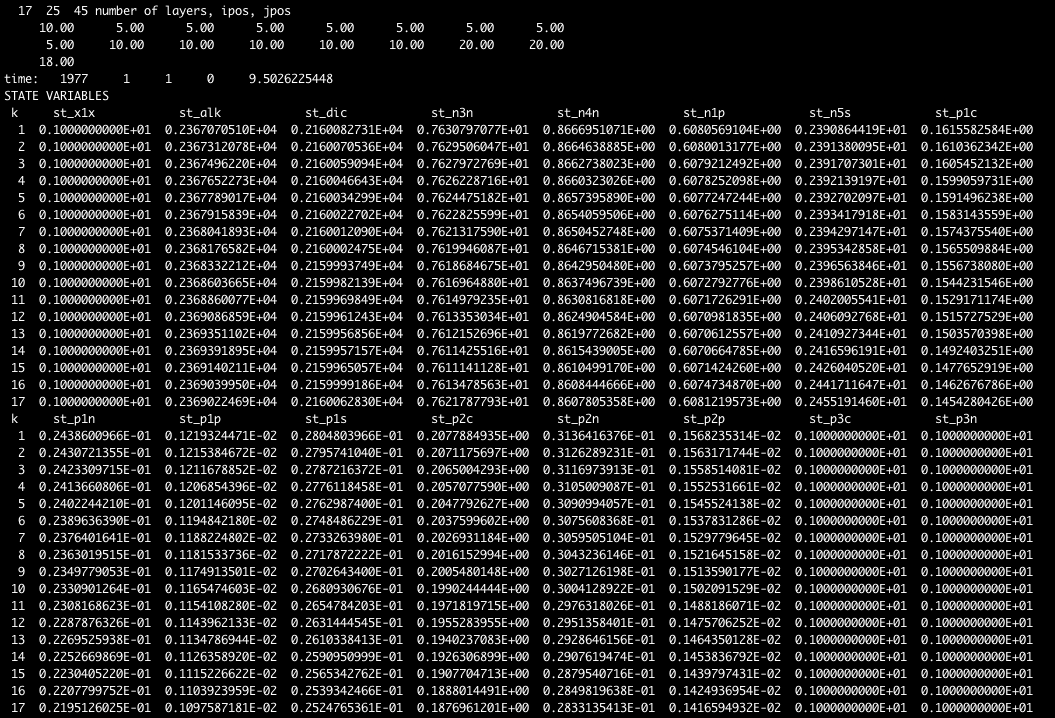
\includegraphics{pics/ncdumpecoham.png}
    \caption{ECOHAM5 with ncdump}
\end{figure}

\begin{figure}[h!]
    \centering
    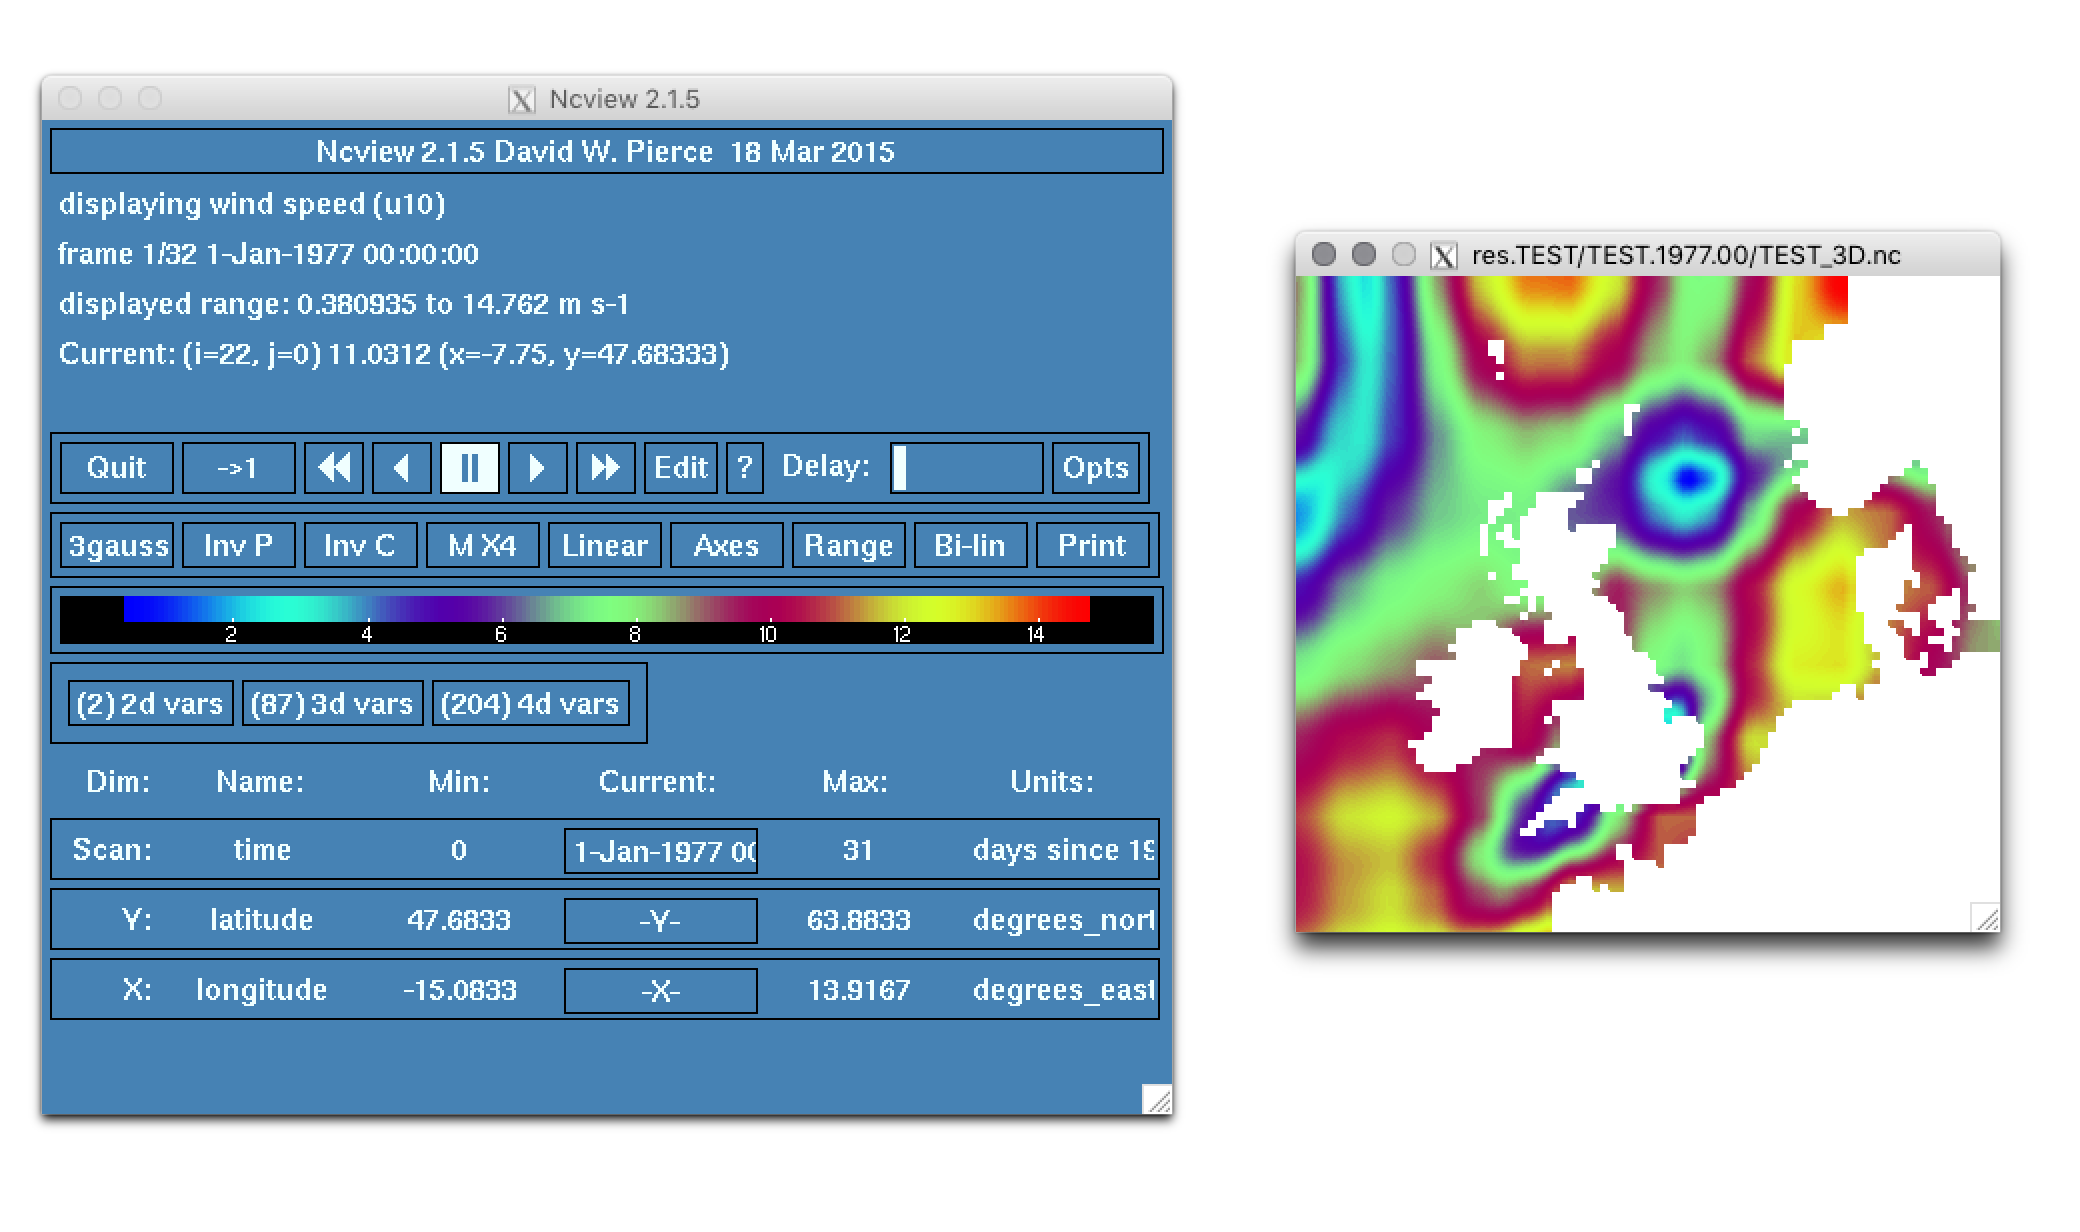
\includegraphics{pics/ncviewecoham.png}
    \caption{Visualization of ECOHAM5 output data in ncview visual browser}
\end{figure}

\section{Life cycle of data}\label{life-cycle-of-data}

\subsection{General}\label{general}

Through the whole process of running a simulation there are different
types of data at certain points. The complexity and the information can
differ. The data which is fed into the program at the beginning won't be
the same which is visualized by a color on the climate overview.
\cite{lanuni}

The life cycle could be divided into the parts shown in \emph{Figure 4}
\cite{lanuni2} and can differ from institution to institution:

\begin{enumerate}
\def\labelenumi{\arabic{enumi}.}
\tightlist
\item
  creating data
\item
  processing data (pre- and post-processing included)
\item
  analyzing data
\item
  preserving data
\item
  giving access to data
\item
  re-using data
\end{enumerate}

\begin{figure}
\centering
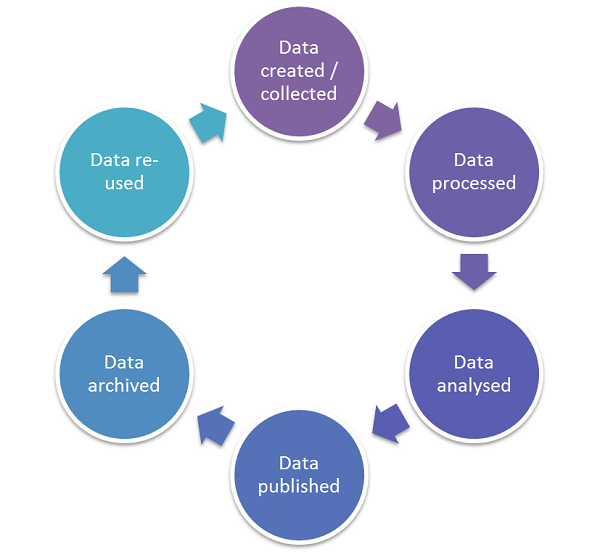
\includegraphics{pics/DataLifecycle.png}
\caption{Data life cycle}
\end{figure}

\subsubsection{Creating the data}\label{creating-the-data}

Creating the data could also be referred to as the design of the
research. The choices made during this step will be crucial, because it
will have an huge impact on the processing as well as at the overall
structure of the application. Which kind of data management, formats or
storage should be used are just some examples of questions which needs
to be answered for a proper design. If there are already similar
existing simulations, their data could be re-used for the current step.
In case there is no similar simulation, new data needs to be collected
by research and experiments. Running simulations and capturing metadata
are important parts of this process.

\subsubsection{Processing data}\label{processing-data}

This step will contain the digitization, transcribing and translation of
data into a useful figure. It also is about the vetting of validate and
clean data. Anonymizing data could also be part of processing. Sometimes
there is pre- and post-processing besides the general processing.
Pre-processing will prepare the particular data before a certain step.
In this step all unneeded information will be dismissed to save time and
storage capacity. After this there might be the post-processing. This
process includes the treatment of data to make it usable for following
steps. For example the data should be described and explained to make it
easy to read for other people. As a last step it is necessary to take a
look at the storage of the data.

\subsubsection{Analyzing of data}\label{analyzing-of-data}

It is hard to get any valuable information out of pure data, especially
if there are thousands of values and rows. Therefore we need methods to
interpret them. Derivation of data during calculation of the output of
the research and making publications is another part. Now main
calculations of the data are done, the data have to be prepared for
preservation.

\subsubsection{Preserving of data}\label{preserving-of-data}

Preservation of data is about looking for the best formats and best
media on which it should be backed up and stored. Also creation of meta
data and documentation is important for the final archiving.

\subsubsection{Giving access to data}\label{giving-access-to-data}

Because research is done mostly by public institutes there is the demand
of sharing and distributing the data and knowledge. Considering a
mechanism for access control and determine copyrights might also be very
useful.

\subsubsection{Re-using data}\label{re-using-data}

Research in the future could also be based on the work which was done in
the past. Teaching and publications may be good examples for re-using.

\subsection{Summary}\label{summary}

With the growth of data in simulations and the constant rapid
improvement of processing power, it is very essential for research
establishments to maintain a proper storage technology. The data and
knowledge are the key and the only thing those institutes are working
for. Therefore data and knowledge needs the right treatment.

\section{Conclusion}\label{conclusion-1}

This project was about the analysis of input and output of climate
applications. We made our way through running models provided by our
supervisors and some we found in the internet which seemed suitable for
our purpose. We faced bad documentations and insufficient scripts for
making such a model run. At the end we didn't manage to run most of them
at different levels of progress. \emph{ECOHAM5} was the only one which
worked on the fly Apart of that it didn't kept us away from documenting
our respective progress on the models as well as analyzing the life
cycle of data in general.

\section{References}\label{references}

\printbibliography

\end{document}
